\section{Basics}

\subsection{Evolutionary Algorithms} \label{sec:EA}

Evolutionary algorithms are population-based metaheuristics \cite{EA}. Metaheuristics are methods for solving optimization problems by iteratively improving candidate solutions in relation to a given quality measure.
Population-based metaheuristics use populations of multiple solutions and iteratively change populations to find a good solution.
An evolutionary algorithm is based on a population $P$ of possible solutions $e_i \in P$ for the optimization problem or heuristic to be solved. A solution is also referred to as an individual in the context of population-based metaheuristics.

In general, evolutionary algorithms consist of the following steps \cite{EA}:

\begin{enumerate}
\item Initialization: The initial population of individuals is generated randomly.

\item Evolutionary process: The individuals are evaluated by calculating their fitness. Therefore a fitness function is needed.
According to their fitness, some of the individuals are selected to be the parents of the following generation.
Then a process with reproduction, recombination, and mutation starts - similar to biological processes.
The parents are being recombinated and the resulting individuals are mutated to form the offspring of the current generation.
These steps are being repeated until a new population of individuals is generated. The parents are also added to the new population. This new population substitutes the old population and the process is repeated until an abort criterion is fulfilled  (see figure \ref{fig:EA}).

\item The best individual is selected.
\end{enumerate}


\begin{figure}
	\begin{center}
		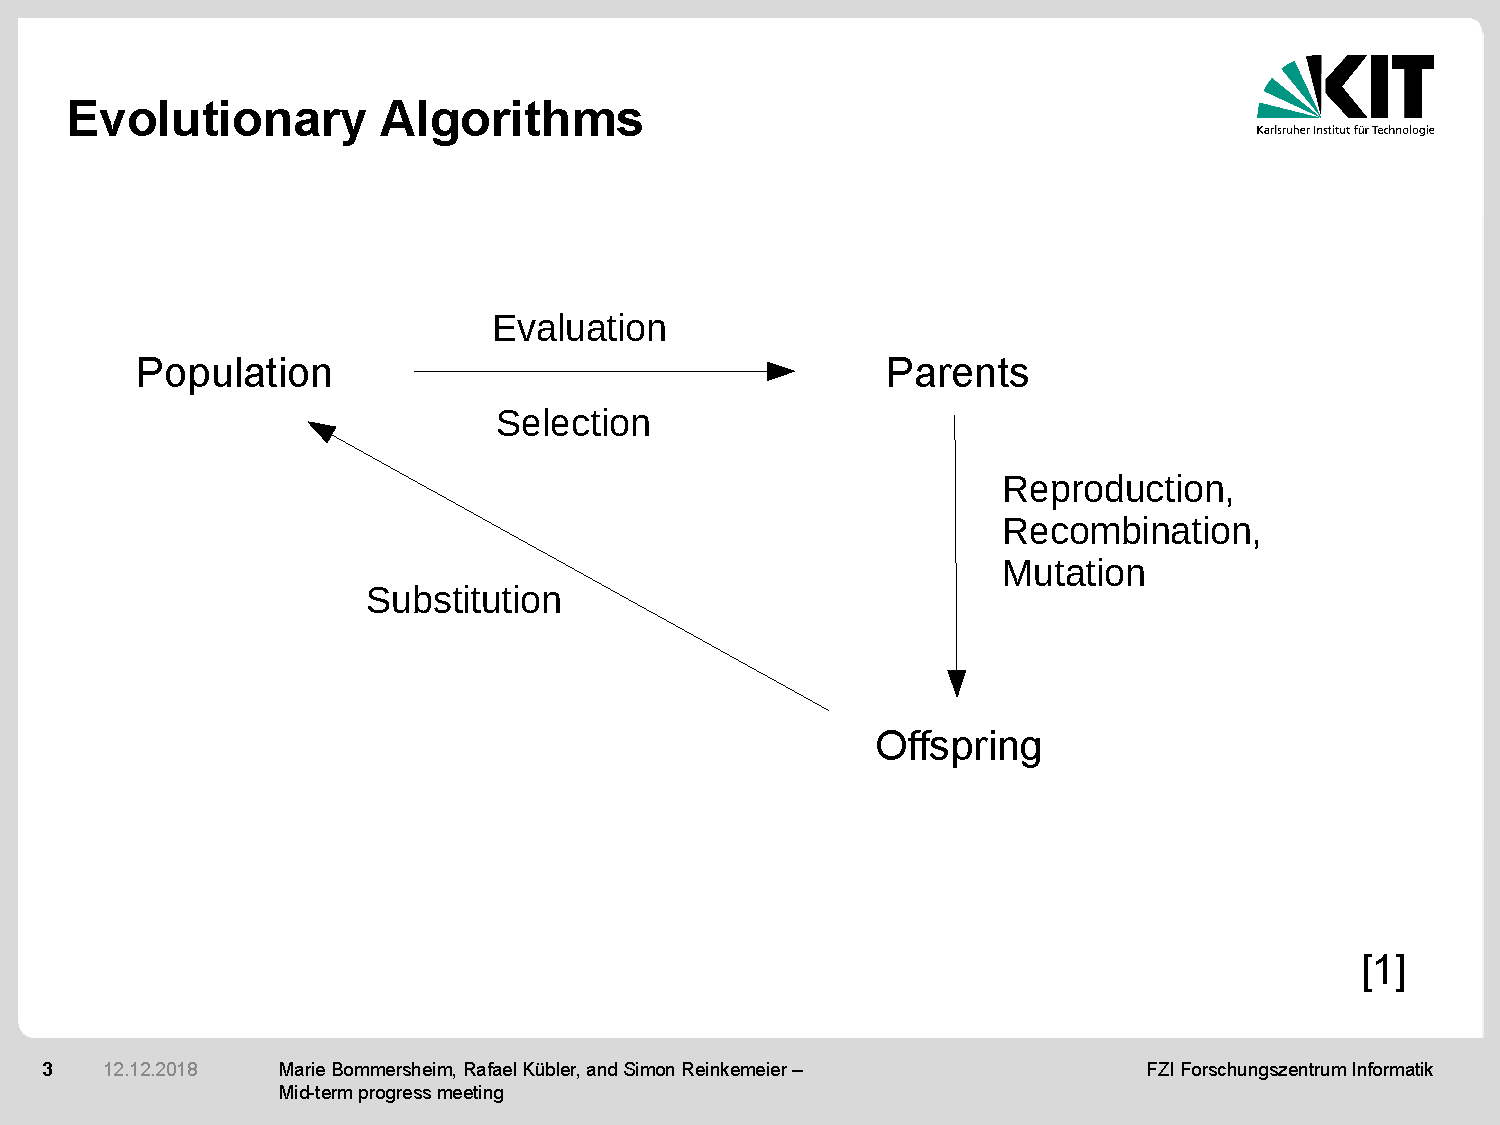
\includegraphics[trim = 2.2cm 6cm 4.1cm 6cm, clip, width=0.4\textwidth]{EA}
	\end{center}
	\caption{Evolutionary algorithms, adapted from \cite{EA}}
	\label{fig:EA}
\end{figure}

\subsection{Monte Carlo Markov Chain} \label{sec:MCMC}

Monte Carlo Markov Chain algorithms can be used for hard optimization problems. The idea is to construct a Markov Chain that generates samples such that more time is spent (more samples are evaluated) in the most interesting regions of the state space (see figure \ref{fig:MCMC1}) \cite{MCMC}. The decision to accept or reject a proposal to go from Point 1 to Point 2 is based on the ratio of posterior densities of the two points: uphill steps are always accepted, small downhill steps are usually accepted but huge downhill steps are almost never accepted (see figure \ref{fig:MCMC2}). 


\begin{figure}
	\begin{center}
		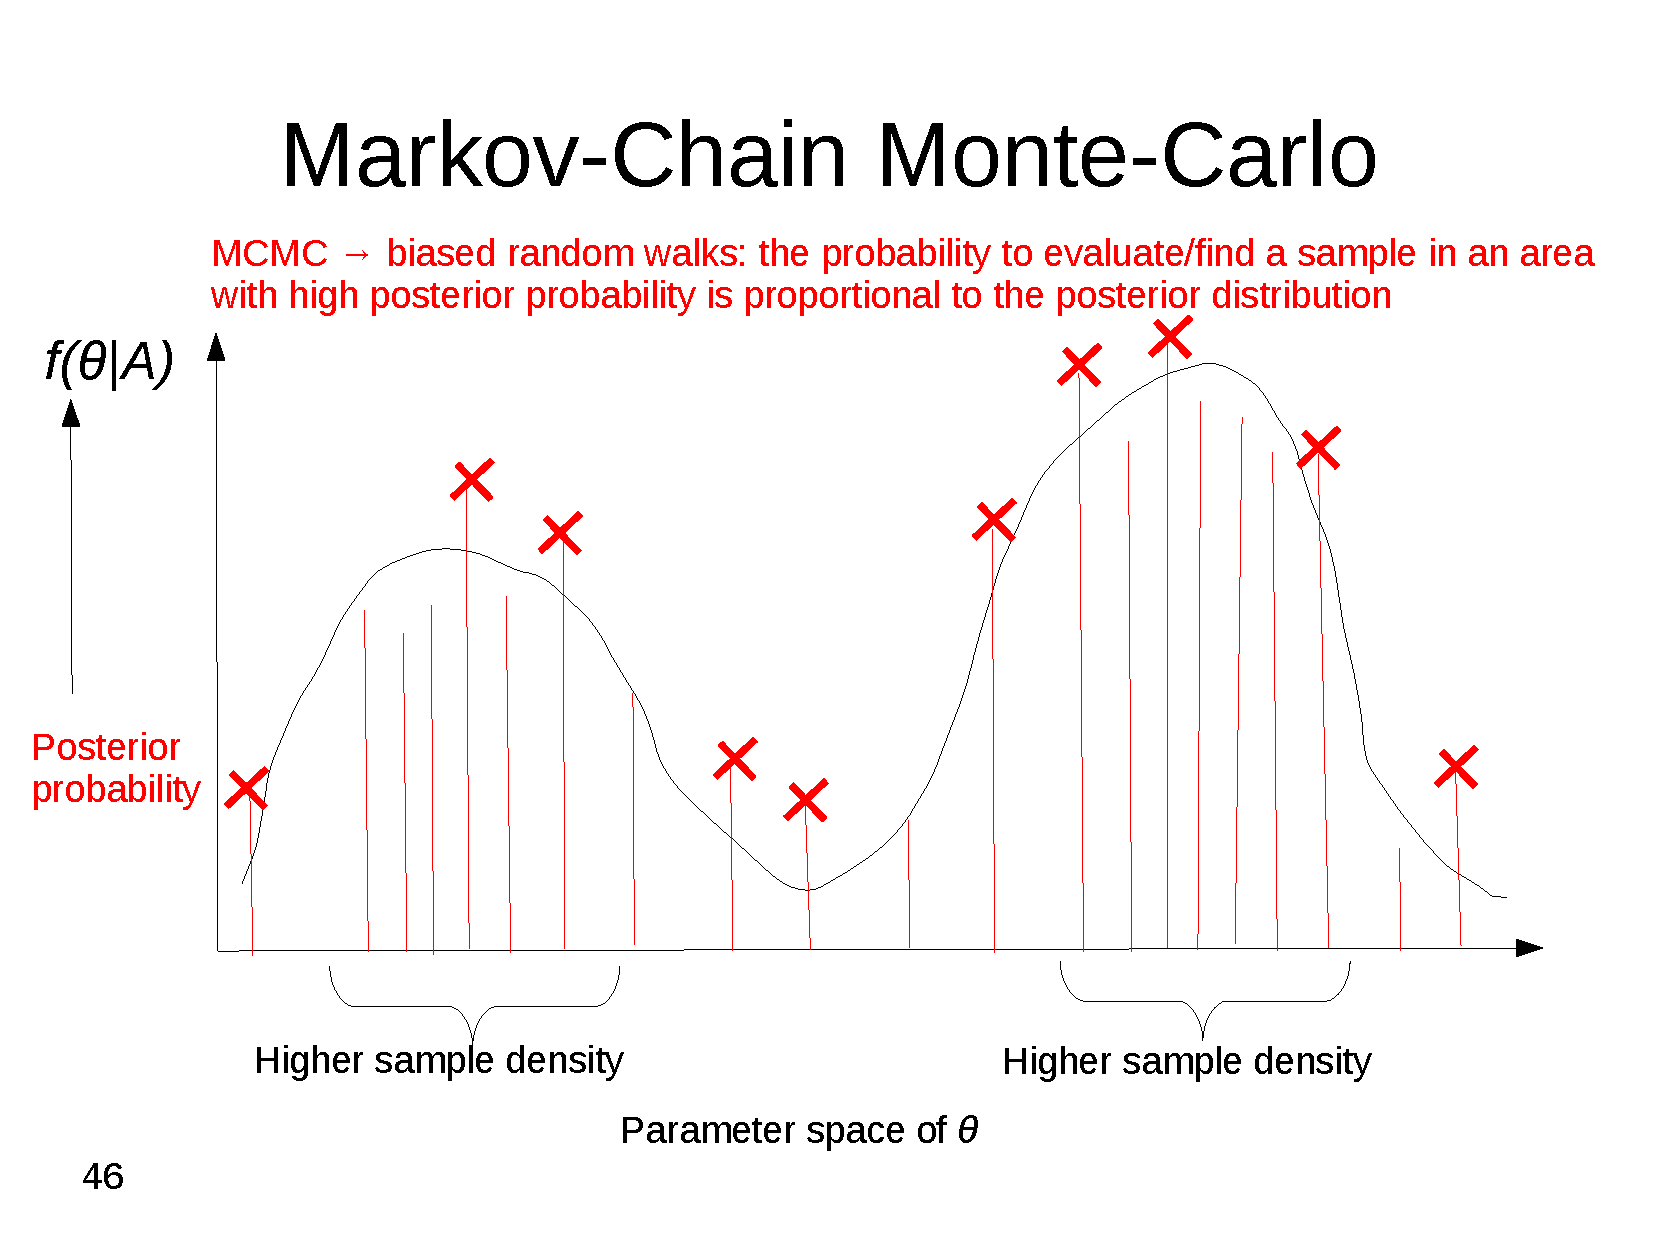
\includegraphics[trim = 0cm 1.5cm 1cm 5.4cm, clip, width=0.4\textwidth]{lecture12-seiten-46}
	\end{center}
	\caption{The probability to evaluate or find a sample in an area with high posterior probability is proportional to the posterior distribution, from \cite{MCMC}}
	\label{fig:MCMC1}
\end{figure}

\begin{figure}
	\begin{center}
		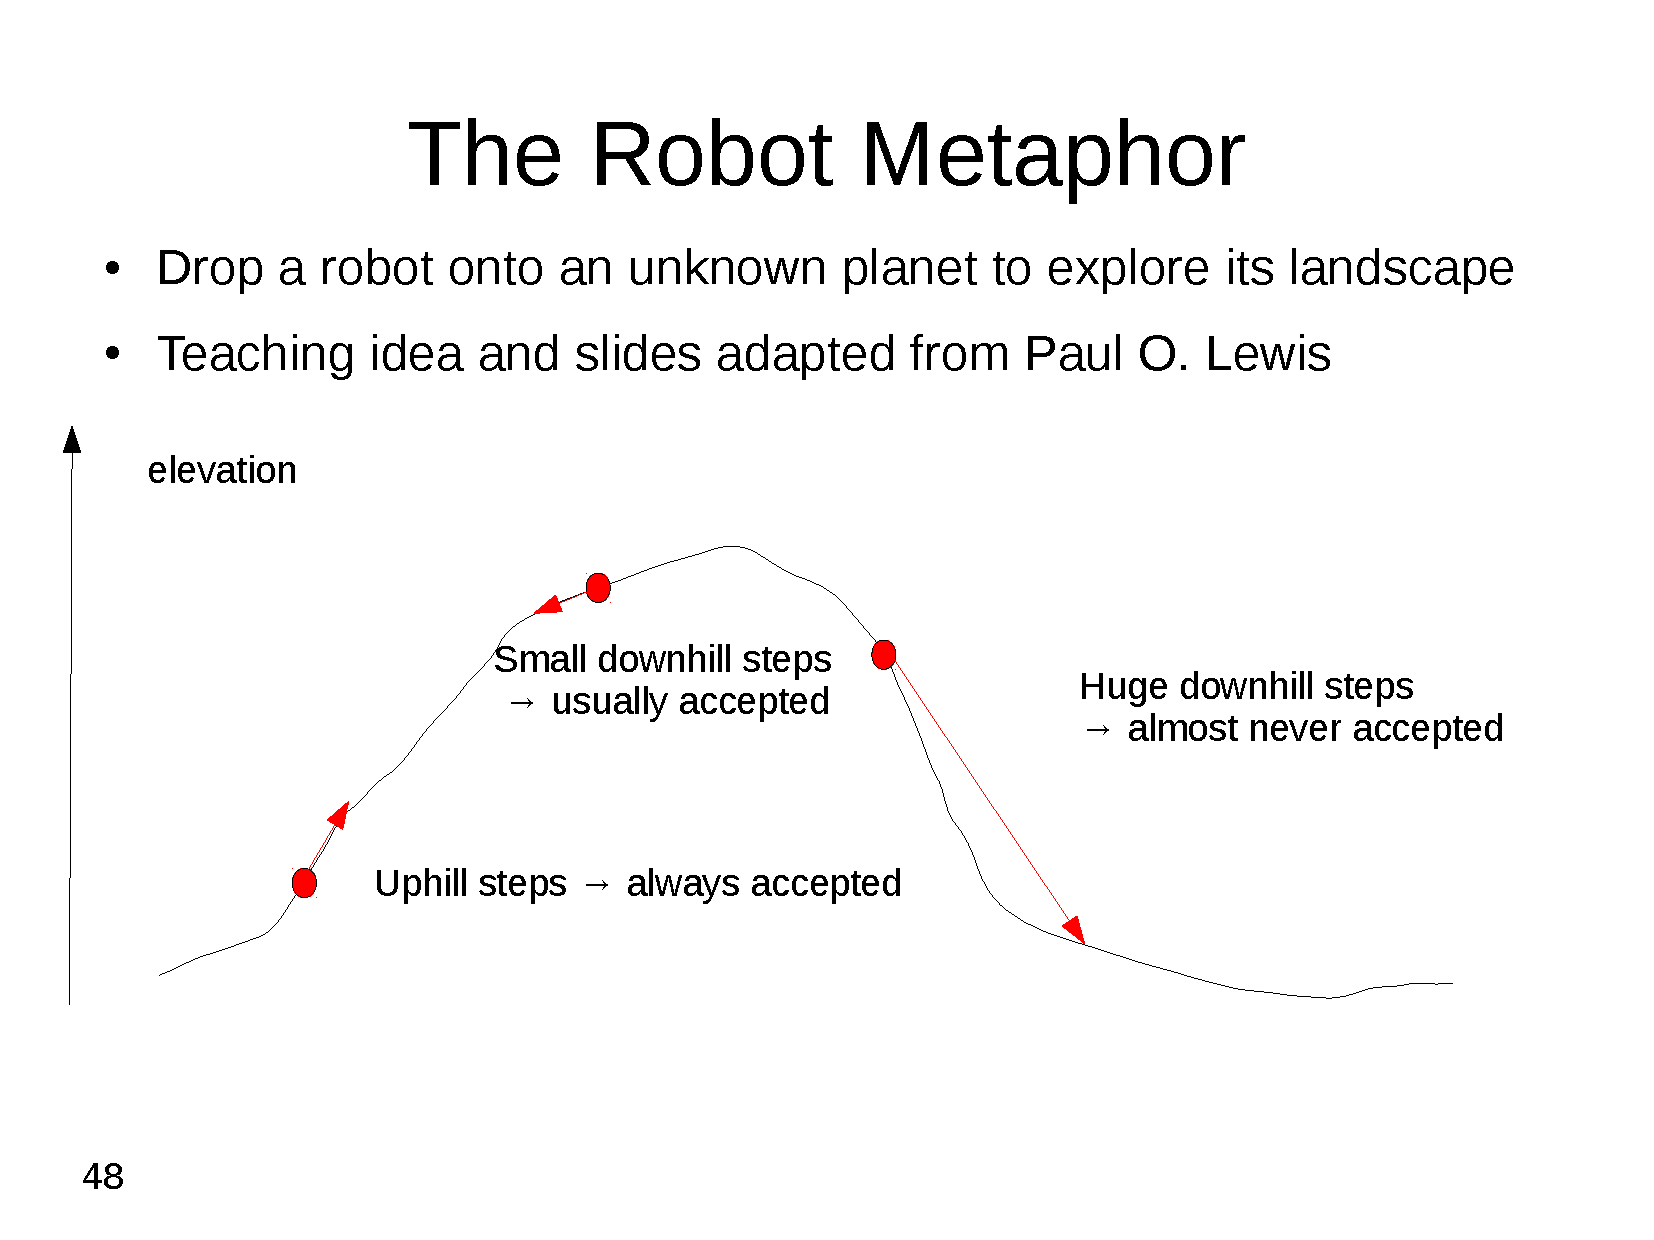
\includegraphics[trim = 0cm 4cm 1cm 7cm, clip, width=0.4\textwidth]{lecture12-seiten-48}
	\end{center}
	\caption{The decision to accept or reject a proposal to go from Point 1 to Point 2 is based on the ratio of posterior densities of the two points/samples, from \cite{MCMC}}
	\label{fig:MCMC2}
\end{figure}